% Slides for TSD day

\documentclass[usenames,dvipsnames]{beamer} % oral talk
%\documentclass[trans]{beamer}  % paper version
\mode<presentation> {
  %\usetheme{Darmstadt}
  \usetheme{Madrid}
  \usecolortheme{crane}
  %\usetheme{Goettingen}
  %\usecolortheme{wolverine}
  \setbeamercovered{transparent}
  %\useoutertheme{sidebar}
}

%Use this one for VERIMAG special barco
\setbeamercolor{frametitle}{bg=Goldenrod}
\setbeamercolor{block title}{bg=Goldenrod}


\usepackage{graphicx}
\usepackage{xspace}
\usepackage[dvips]{epsfig}
\usepackage{xmpmulti}
\usepackage{color}
\usepackage{colortbl}
\usepackage{setspace}
\usepackage{array}
\usepackage{latexsym}
\usepackage{comment}
\usepackage{amssymb,amsmath,amsthm}
\usepackage{ulem}
\usepackage{extarrows}

\usepackage {bussproofs}
\bottomAlignProof

\usepackage{dednatcol}
\usepackage{alltt}
\usepackage[latin1]{inputenc}
\usepackage{times}
\usepackage[T1]{fontenc}
\usepackage[english]{babel}

\definecolor{Blue}{rgb}{0.1,0.1,0.8}

\newcommand{\keywd}[1]{\textbf{#1}}

\setbeamercovered{dynamic}
\setbeamertemplate{theorems}[numbered]

\newcommand{\hs}{\hspace{1cm}}
\newcommand{\vs}{\vspace{1cm}}
\newcommand{\vsfive}{\vspace{5mm}}
\newcommand{\hsfive}{\hspace{5cm}}

\newcommand{\mboxfill}{\mbox{ }\hfill}

% Variables logiques

\newcommand{\rv}{\bleu {rv}\xspace}
\newcommand{\re}{\bleu {re}\xspace}
\newcommand{\rg}{\bleu {rg}\xspace}
\newcommand{\rd}{\bleu {rd}\xspace}

\newcommand{\pv}[1]{{\bleu {\textsf{I}}(\marron{#1})}}
\newcommand{\pe}[1]{{\bleu {\textsf{W}}(\marron{#1})}}
\newcommand{\pg}[1]{{\bleu {\textsf{S}}(\marron{#1})}}
\newcommand{\pd}[1]{{\bleu {\textsf{D}}(\marron{#1})}}

\newcommand{\vv}[1]{{\bleu {I}(\ensuremath{\vav{#1}})}}
\newcommand{\ve}[1]{{\bleu {W}(\ensuremath{\vav{#1}})}}
\newcommand{\vg}[1]{{\bleu {S}(\ensuremath{\vav{#1}})}}
\newcommand{\vd}[1]{{\bleu {D}(\ensuremath{\vav{#1}})}}

\newcommand{\mystrut}{\hbox to 0pt{\phantom{()}}}
%%%%%%%%%%%%%%%%%


\newtheorem{defn}{Definition}


%\newtheorem{theo}{Theorem}[section] % theorems are numbered by section
\newtheorem{theo}{Theorem} % theorems are numbered by section
\newtheorem{prop}[theo]{Proposition} % propositions are numbered as theorems
\newtheorem{lem}{Lemma} % lemmas are no longer numbered as theorems
\newtheorem{myfact}[theo]{Fact} % lemmas are numbered as theorems
\newtheorem{de}[theo]{Definition} % 

% \newcommand{\egdef}%
%    {\ensuremath{~\:\mathrel{\raisebox{-.7ex}%
%    {$\stackrel{\rm def}{=\mkern-8mu=}$}}\:~}}

\renewcommand{\impl}{\ensuremath{\Rightarrow}}


% \definecolor{marron}{rgb}{0.6, 0.2, 0}
% \definecolor{mygreen}{rgb}{0.0,0.5,0.0}
% \definecolor{brique}{rgb}{0.75, 0.05, 0}
% \definecolor{violet}{rgb}{.75, 0, .75}

% \definecolor{lightblue}{rgb}{0.75,0.85,1}
% \definecolor{lightred}{rgb}{1,0.8,0.8}
% \definecolor{lightgreen}{rgb}{0.6,1,0.6}
% \definecolor{semilightgreen}{rgb}{0.5,1,0.5}
% \definecolor{lightyellow}{rgb}{1.0,1.0,0.5}
% \definecolor{lightorange}{rgb}{1.0, 0.87, 0.01}

% \newcommand{\marron}[1]{\textcolor{marron}{#1}}
% \newcommand{\brun}[1]{\textcolor{brown}{#1}}
% \newcommand{\cvert}[1]{\textcolor{mygreen}{#1}}
% \newcommand{\bleu}[1]{\textcolor{blue}{#1}}
% \newcommand{\rouge}[1]{\textcolor{red}{#1}}
% \newcommand{\brique}[1]{\textcolor{brique}{#1}}
% \newcommand{\violet}[1]{\textcolor{violet}{#1}}

\newcommand{\cdat}{\violet}
\newcommand{\cloc}{\cvert}

% ----------------------------------------------------------------------
\newcommand{\loc}{\cloc{\textit{loc}}}
\newcommand{\lx}{\cloc{\textit{x}}}
\newcommand{\ly}{\cloc{\textit{y}}}

\newcommand{\edge}[2]{\ensuremath{\cloc{#1\!\mathbin{\rightarrow}\! #2}}}
\newcommand{\cdb}{\ensuremath{\mathcal{\cdat C}}}
\newcommand{\incdb}[1]{\ensuremath{#1\in\cdb}}
\newcommand{\nincdb}[1]{\ensuremath{#1\not\in\cdb}}
\newcommand{\cdbp}{\ensuremath{\cdat{\mathcal{C}'}}}
\newcommand{\incdbp}[1]{\ensuremath{#1\in\cdbp}}
\newcommand{\nincdbp}[1]{\ensuremath{#1\not\in\cdbp}}
\newcommand{\atloc}[1]{\cdat{\ensuremath{\left|\cloc{#1}\right|}}}
\newcommand{\inset}[2]{\ensuremath{#1\in#2}}
\newcommand{\inloc}[2]{\ensuremath{#1\in\atloc{#2}}}
\newcommand{\ninloc}[2]{\ensuremath{#1\not\in\atloc{#2}}}
\newcommand{\visloc}[2]{\ensuremath{#1\in\cdat{\overline{\atloc{#2}}}}}
\newcommand{\nvisloc}[2]{\ensuremath{#1\not\in\cdat{\overline{\atloc{#2}}}}}
\newcommand{\inedge}[3]{\inloc{#1}{\edge{#2}{#3}}}
\newcommand{\ninedge}[3]{\ninloc{#1}{\edge{#2}{#3}}}
\newcommand{\cnf}{\textit{\cdat{cnf}}}
\newcommand{\pre}{\cdat{\textit{pre}}}
\newcommand{\post}{\cdat{\textit{post}}}
\newcommand{\extconfpar}[2]{\cdat{\ensuremath{\langle #1, #2\rangle}}}
\newcommand{\extconf}{\extconfpar{\cnf}{\cdb}}
\newcommand{\extconfpre}{\extconfpar{\pre}{\cdb}}
\newcommand{\extconfpost}{\extconfpar{\post}{\cdbp}}
%\newcommand{\entails}{~\rhd~}
\newcommand{\entailstrans}{\:\xrightarrow{\:trans\:}\:} % general
\newcommand{\entailsp}{\:\xrightarrow{\:sr\:}\:} % pure synchronous round
\newcommand{\entailso}{\:\xrightarrow{\:or\:}\:} % oracle round
\newcommand{\entails}{\:\xrightarrow{\:sor\:}\:} % synchronous + oracle round
\newcommand{\roas}{\textsc{roas}}
\newcommand{\roasat}[2]{\ensuremath{\roas\,@\,\edge{#1}{#2}}}
\newcommand{\roasto}[1]{\ensuremath{\roas\,@\,\cloc{\overline{#1}}}}
\newcommand{\goodat}[2]{\ensuremath{good\,@\,\edge{#1}{#2}}}
\newcommand{\goodto}[1]{\ensuremath{good\,@\,\cloc{\overline{#1}}}}
\newcommand{\correctonSTat}[1]{\ensuremath{\mbox{correct-onST}\,@\,\cloc{#1}}}
\newcommand{\wcorrectonSTat}[1]{\ensuremath{\mbox{weak-correct-onST}\,@\,\cloc{#1}}}
\newcommand{\completeonSTat}[1]{\ensuremath{\mbox{complete-onST}\,@\,\cloc{#1}}}
\newcommand{\readyat}[1]{\ensuremath{\mbox{ready}\,@\,\cloc{#1}}}
\newcommand{\correctSTat}[1]{\ensuremath{\mbox{correct-ST}\,@\,\cloc{#1}}}
\newcommand{\completeSTat}[1]{\ensuremath{\mbox{complete-ST}\,@\,\cloc{#1}}}
\newcommand{\invarat}[1]{\ensuremath{\mbox{invar}\,@\,\cloc{#1}}}


\newcommand{\hcinv}{\texttt{hc\_inversion}\xspace}


% Front page

\title{Certification of an Instruction Set Simulator}

%\subtitle{No subtitle}
\bigskip
\author[X. Shi] % (optional, nur bei vielen Autoren)
{\large Xiaomu Shi\\\bigskip{\small Supervised by: Jean-Fran\c{c}ois Monin \& Vania Joloboff}}

\institute[LIAMA, VERIMAG \& Univ Grenoble]

\date[July 10th, 2013]

\begin{document}

\frame{\titlepage

\vfill

}

\section<presentation>*{Outline}

\begin{frame}
  \frametitle{Outline}
  %\setcounter{tocdepth}{2}
  \tableofcontents[subsectionstyle=hide]%[part=1,pausesections]
\end{frame}

% \AtBeginSubsection[] {
%   \begin{frame}<handout>
%     \frametitle{Outline}
%     \tableofcontents[sectionstyle=hide,currentsubsection]
%   \end{frame}
% }

\AtBeginSection[] {
  \begin{frame}<beamer>
    \frametitle{Outline}
    \setcounter{tocdepth}{2}
    \tableofcontents[current,subsection]
  \end{frame}
}


%%%%%%%%%%%%%%%%%%%%%%%%%%%%%%%%%%%%%%%%%%%%%%%%%%%
%%%%%%%%%%%%%%%%%%%%%%%%%%%%%%%%%%%%%%%%%%%%%%%%%%%
\section{Introduction}

%%%%%%%%%%%%%%%%%%%%%%%%%%%%%%%%%%%%%%%%%%%%%%%%%%%

\subsection{Certifying C programs}

% JF -> XM: 
% - ref ro model checking somewhat dangerous
%   (your statement on large systems is wrong; what holds is that
%    MC is inadequate for general software managing complex data, e.g. your 3 examples
% - if you want to keep it, say that MC is good at [to be completed, but no mistake!]
% - May be better to just say that for this kind of applications, the approach based on
%   deductive verification was successful in several cases

\begin{frame}
\frametitle{We want to trust our program}
\begin{block}{}
\begin{itemize}

\item \large\brique{Goal: the execution of a program behaves as expected}
\item Approaches based on deductive verification:
  \begin{itemize}
  \item NICTA's Secure Embedded L4 microkernel (Isabelle/HOL), 2009
  \item Formal verified C compiler CompCert (Coq), 2005
  \item AMD verified floating-point division units (ACL2), 2005.\\
    (Nqthm and its successor ACL2 are well adopted by industry, for processors and softwares, 1993 - now)  
  \end{itemize}
\end{itemize}
\end{block}
\end{frame}

\begin{frame}
\frametitle{Popular approach for certifying a C program}
\begin{block}
{Tools based on axiomatic semantics (Hoare logic)}
Frama-C: a platform for C
program static analysis and automatic deductive verification
\end{block}
\bigskip
%\pause
\textcolor{blue}{%
Difficult to express complex specifications and expected
properties at the right abstraction level
}
\end{frame}

\begin{frame}
\frametitle{Using CompCert C for C program certification}
%have not been tried until our approach
\begin{block}
{Operational semantics based approach}
CompCert C: 
\begin{itemize}
\item Coq-certified C compiler (developed at INRIA)
\item \textit{formal semantics of a large subset of C language}
\end{itemize}
\end{block}
\bigskip
%\pause
\textcolor{blue}{%
Accurate and rich enough to express our large specification,\\
containing a formal model of ARMv6 for SimSoC
}
\end{frame}

\begin{frame}
\frametitle{Short introduction on Coq}
\begin{block}{}
\begin{centering}
\cvert{Coq = winner of} \\ 
\cvert{ACM SIGPLAN Programming Languages Software 2013 award}
\end{centering}
\end{block}
\begin{itemize}
\item \bleu{A formal language}: write formal specifications, programs and etc.
\item \bleu{An interactive theorem prover}: use built-in tactics to process user-guided
  proofs and type-check the correctness of proofs.
\end{itemize}
\end{frame}

\begin{frame}
\frametitle{Screen shot of CoqIDE}
\hfil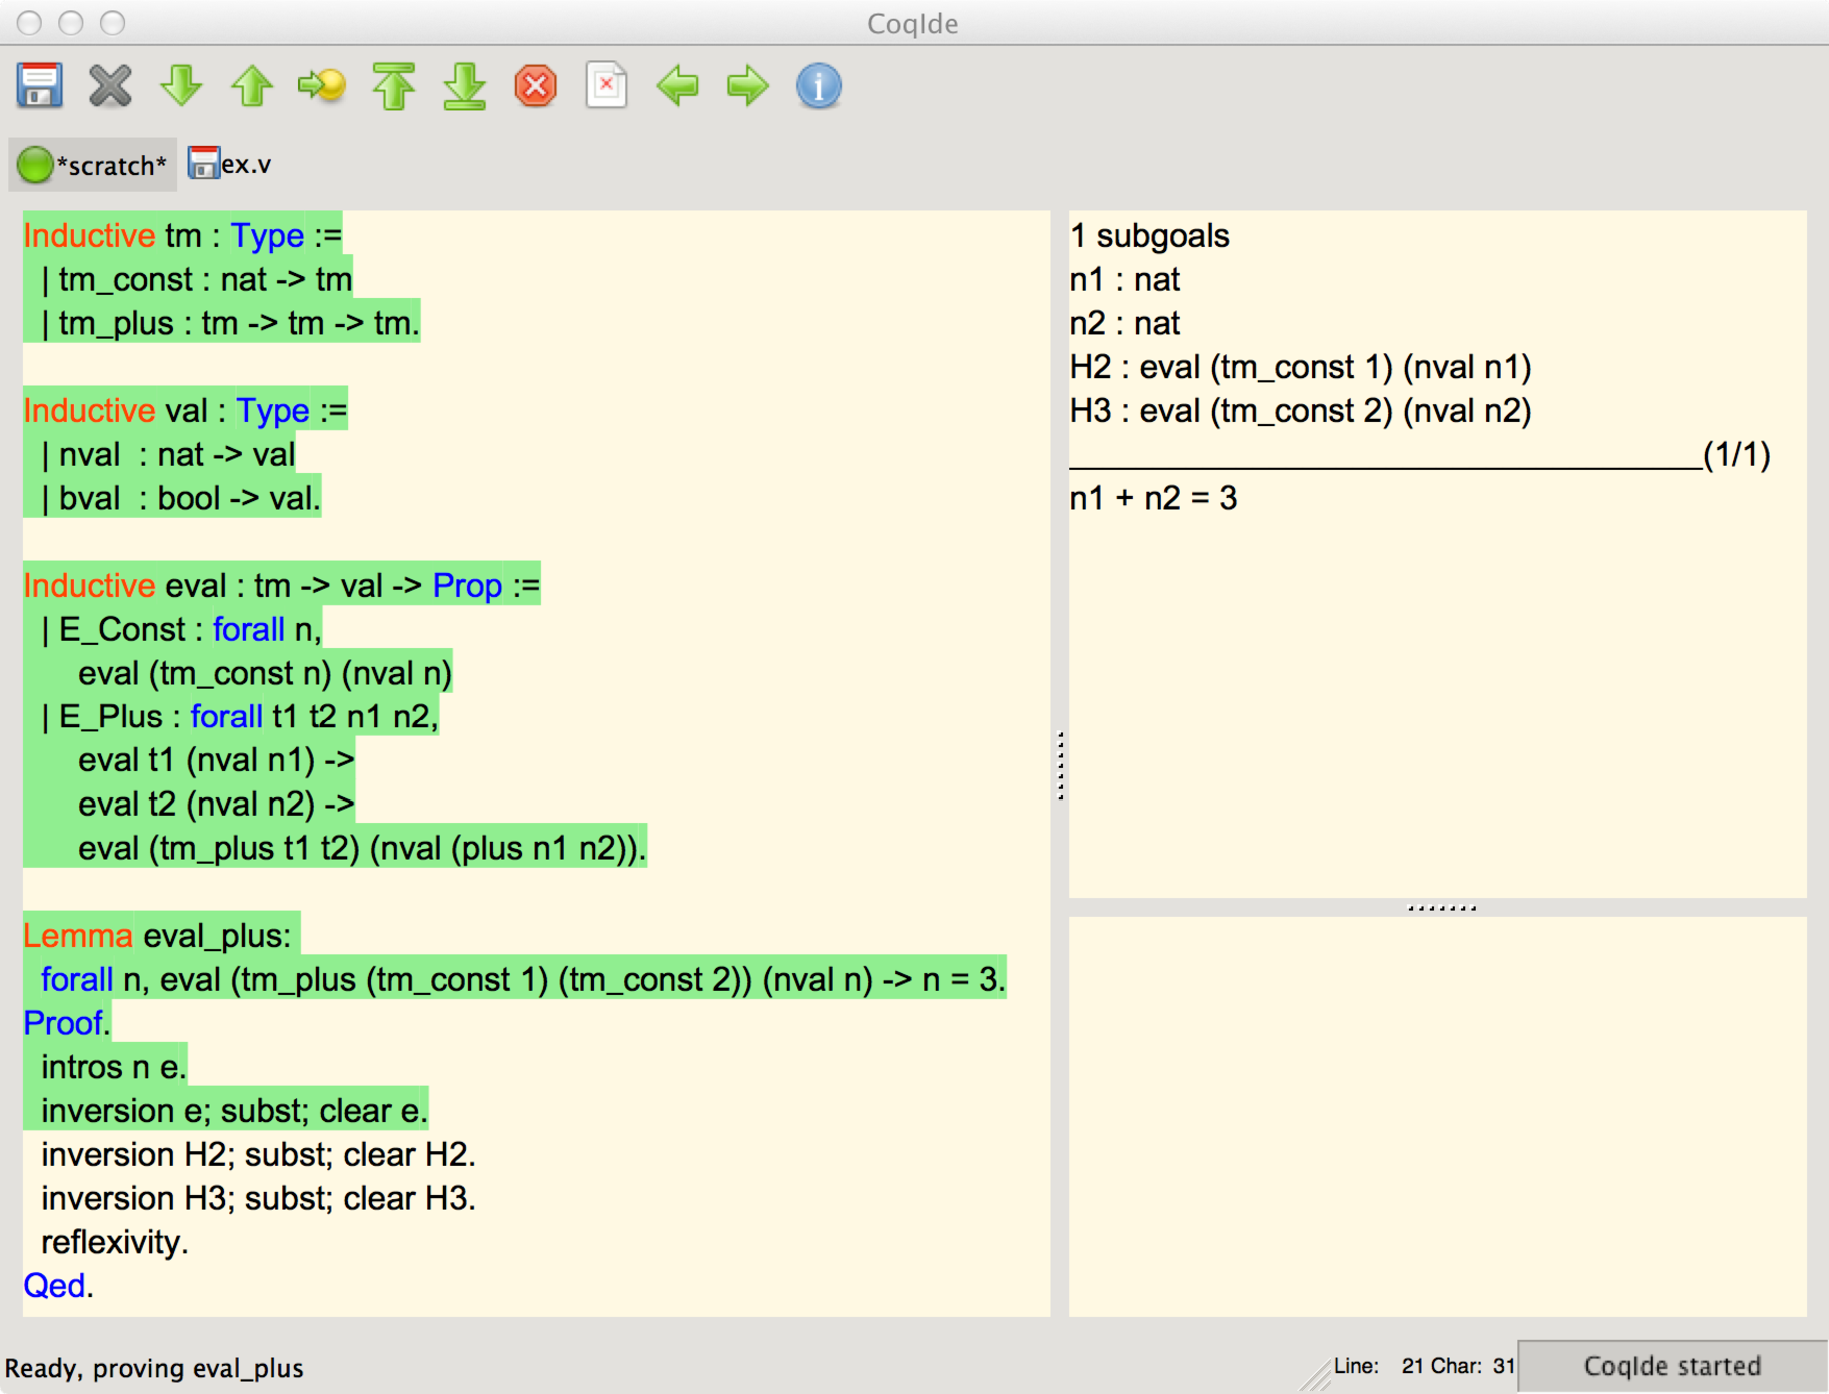
\includegraphics[width=.95\linewidth]{fig/coqide.pdf}
\end{frame}

\subsection{Certification target, SimSoC}

\begin{frame}
\frametitle{The C++ open-source, SimSoC}
\begin{block}{SimSoc: Simulator of System-On-Chip}
Benefits:
\begin{itemize}
\item Time: shorten the development and test phases
\item Cost: no need for a hardware development board
\end{itemize}
\end{block}
\begin{block}{Features}
\begin{itemize}
\item Simulates various architectures: ARM PPC MIPS SH4
\item 60,000 lines of C++ and SystemC
\item Over 100 millions instructions per second
\item Loosely-timed
\item Includes optimizations
\item Can run Linux both on ARM and PowerPC architectures
\end{itemize}
\end{block}
\medskip
\large
\brique{Does the simulator actually simulate the real hardware?}
\end{frame}

\begin{frame}
\frametitle{The ARM simulation module}

\begin{block}{ARM programmer's model}
\begin{itemize}
\item ARM processor
\item 147 ARM instructions
\item 5 kinds of addressing mode
\item System Control Coprocessor (CP15)
\item Memory Management Unit (MMU)
\end{itemize}
\end{block}
\bigskip
ARMv5 simulator was manually implemented
\end{frame}

\begin{frame}
\frametitle{Simlight: a light version in C }
\begin{block}{ARM programmer's model}
\begin{itemize}
\item ARM processor
\item 147 ARM instructions
\item 5 kinds of addressing mode
\item \sout{System Control Coprocessor (CP15)}
\item \sout{Memory Management Unit (MMU)} $\rightarrow$ simplified memory model 
\end{itemize}
\end{block}
\bigskip
Functions for simulating ARMv6 instructions automatically generated
\end{frame}


%%%%%%%%%%%%%%%%%%%%%%%%%%%%%%%%%%%%%%%%%%%
\section{SimSoC-Cert}

%%%%%%%%%%%%%%%%%%%%%%%%%%%%%%%%%%%%%%%%%%%

\subsection{Overall architecture of SimSoC-Cert}
\begin{frame}
\frametitle{Overall architecture of SimSoC-Cert}
\hfil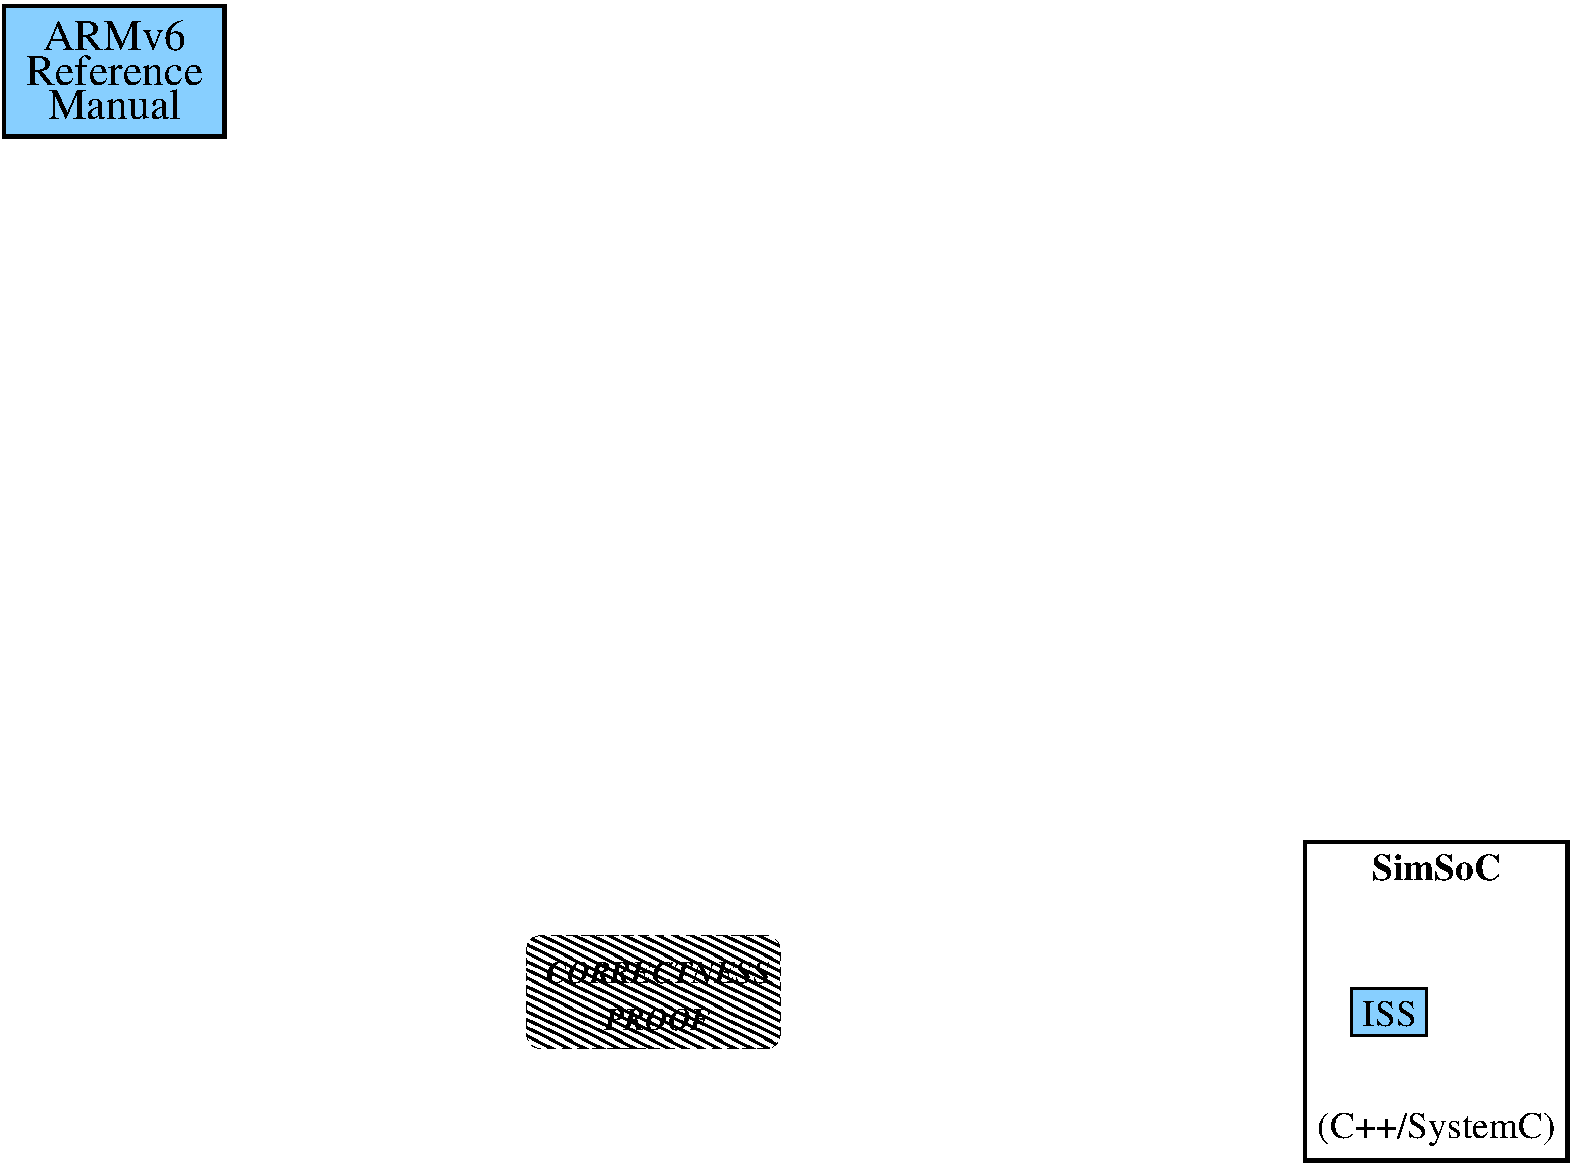
\includegraphics[width=.9\linewidth]{fig/maingen.pdf}
\end{frame}

\begin{frame}
\frametitle{Overall architecture of SimSoC-Cert}
\hfil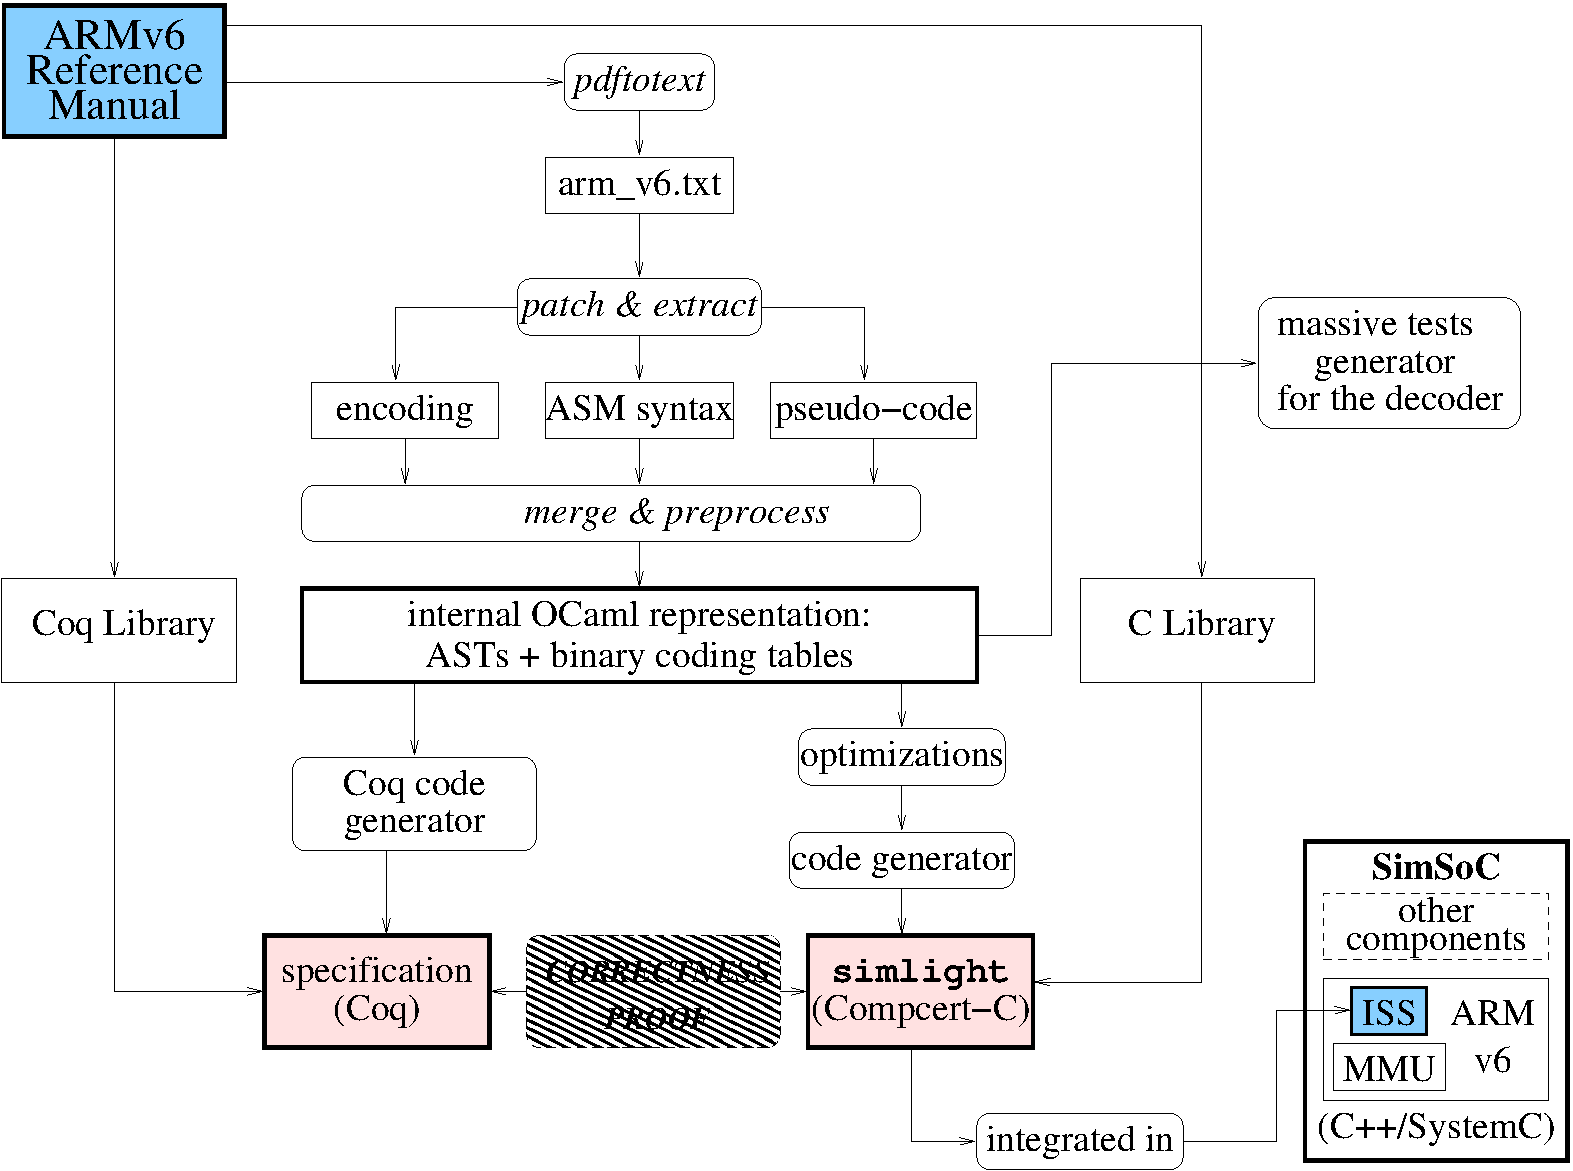
\includegraphics[width=.9\linewidth]{fig/fullarchi.pdf}
\end{frame}

\begin{frame}
\frametitle{My contribution}
\hfil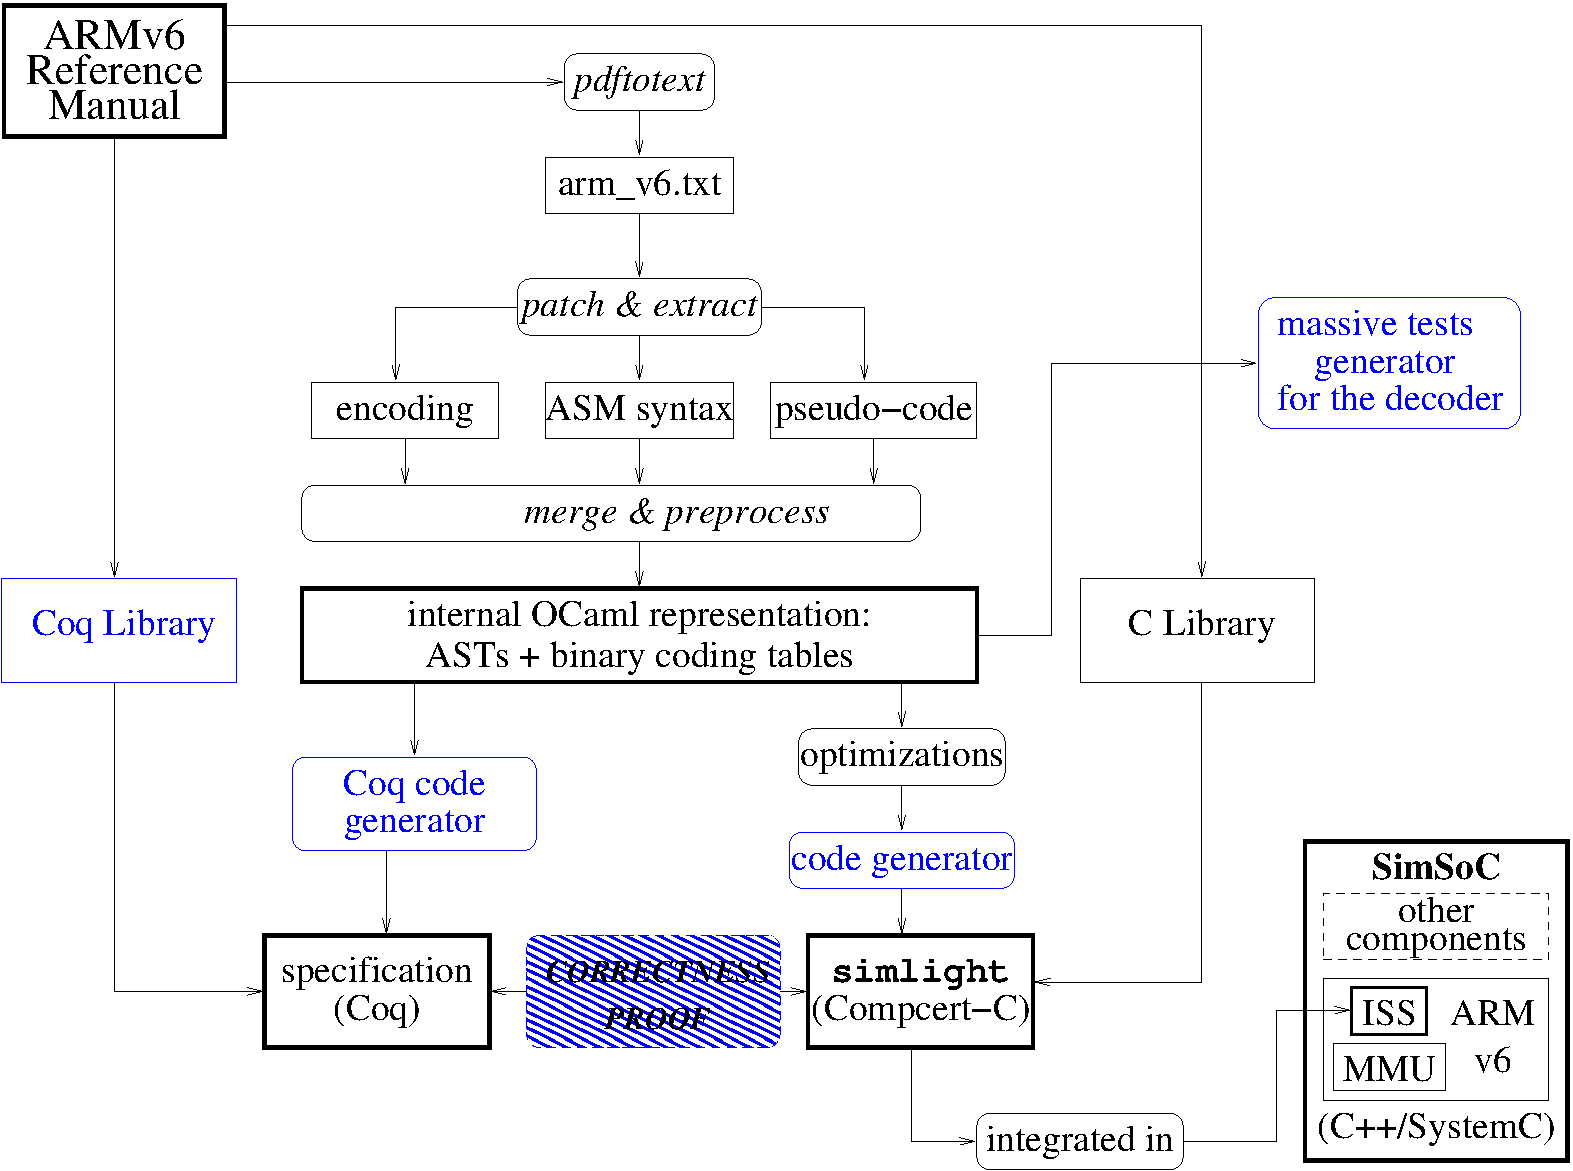
\includegraphics[width=.9\linewidth]{fig/mypart.pdf}
\end{frame}
\subsection{ARM model}

\begin{frame}
\frametitle{ARMv6 ref manual: instruction ADC in pseudo-code}
\hfil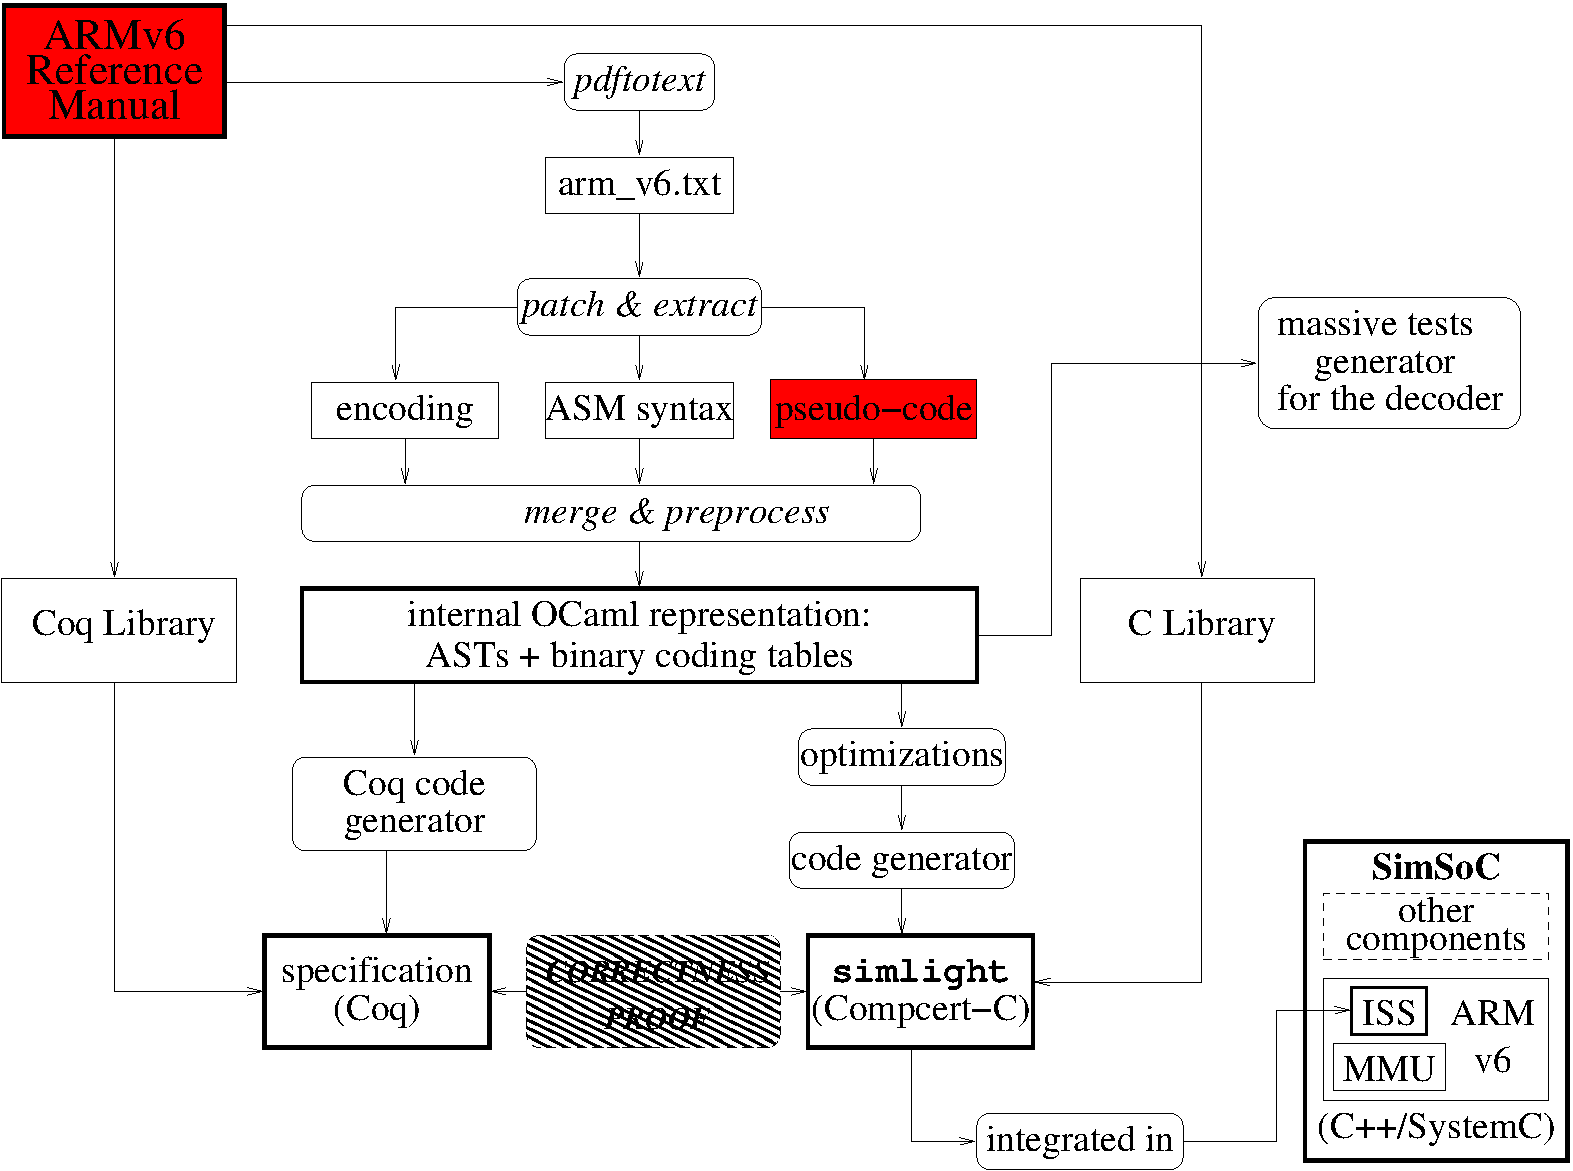
\includegraphics[width=.9\linewidth]{fig/highlight_ref.pdf}
\end{frame}

\begin{frame}[fragile]
\frametitle{ARMv6 ref manual: instruction ADC in pseudo-code}
%code of ADC
\begin{alltt}
A4.1.2 ADC
  \bleu{if} ConditionPassed(cond) \bleu{then}
    \textbf{Rd = Rn + shifter_operand + C Flag;}
    \bleu{if} S == 1 and d == 15 \bleu{then}
      \bleu{if} CurrentModeHasSPSR() \bleu{then}
          CPSR = SPSR;
      \bleu{else} UNPREDICTABLE
    \bleu{else} \bleu{if} S == 1 \bleu{then}
      N Flag = Rd[31];
      Z Flag = \bleu{if} Rd == 0 \bleu{then} 1 \bleu{else} 0;
      C Flag = CarryFrom(Rn + shifter_operand
                            + C Flag);
      V Flag = OverflowFrom(Rn + shifter_operand
                               + C Flag);

\end{alltt}
\end{frame}

\begin{frame}
\frametitle{Coq specifications of ARM instruction ADC}
\hfil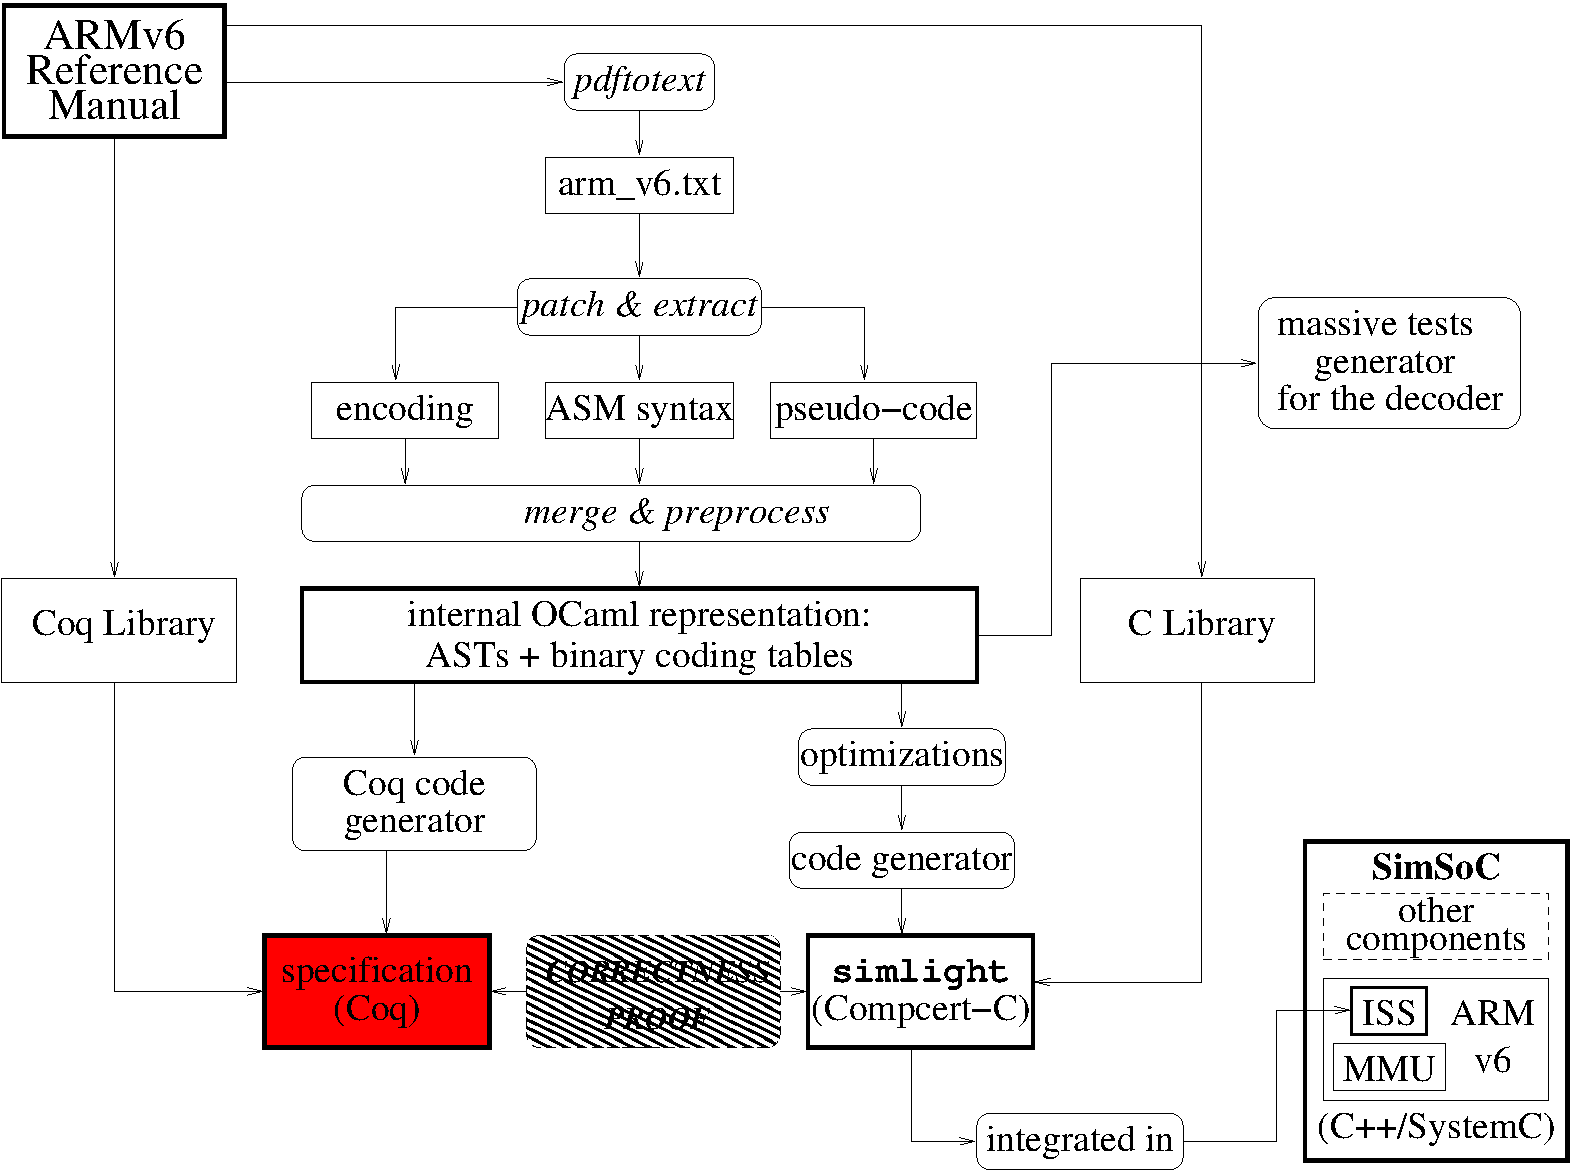
\includegraphics[width=.9\linewidth]{fig/highlight_abstract.pdf}
\end{frame}

\begin{frame}
\frametitle{The state of the abstract model}
\begin{center}
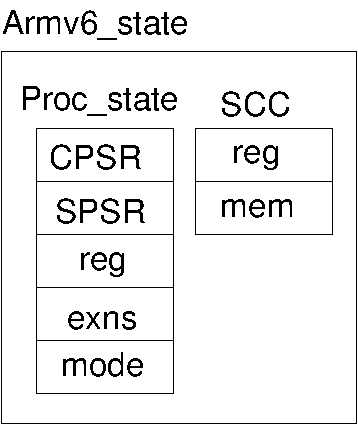
\includegraphics[width=.4\linewidth]{fig/abstr_st.pdf}
\end{center}
\end{frame}

\begin{frame}[fragile]
\frametitle{Coq specification of ARM instruction ADC}
\small
\begin{alltt}
(* A4.1.2 ADC *)
Definition ADC_step
    (S : bool) (cond : opcode) (d : regnum) (n : regnum)
    (shifter_operand : word) : semfun _ := 
  \brique{<s0>} \bleu{if}_\bleu{then} (ConditionPassed s0 cond)
    ([ \brique{<st>} set_reg d (add (add (reg_content s0 n)
                                shifter_operand)
                                ((cpsr st)[Cbit]))
    ; \bleu{If} (andb (zeq S 1) (zeq d 15))
       \bleu{then}
           (\brique{<st>} if_CurrentModeHasSPSR (fun em =>
              (\brique{<st>} set_cpsr (spsr st em))))
\tiny
            \bleu{else}         (\bleu{if_then} (zeq S 1)
                ([ \brique{<st>} set_cpsr_bit Nbit ((reg_content st d)[n31])
                ; \brique{<st>} set_cpsr_bit Zbit (\bleu{if} zeq (reg_content st d) 0 \bleu{then} repr 1 
                                          \bleu{else} repr 0)
                ; \brique{<st>} set_cpsr_bit Cbit
                          (CarryFrom_add3 (reg_content s0 n) shifter_operand
                                          ((cpsr st)[Cbit]))
                ; \brique{<st>} set_cpsr_bit Vbit (OverflowFrom_add3 (reg_content s0 n)
                                     shifter_operand ((cpsr st)[Cbit])) ])) ]).
\end{alltt}
\end{frame}


\begin{frame}
\frametitle{C code of ARM instruction ADC}
\hfil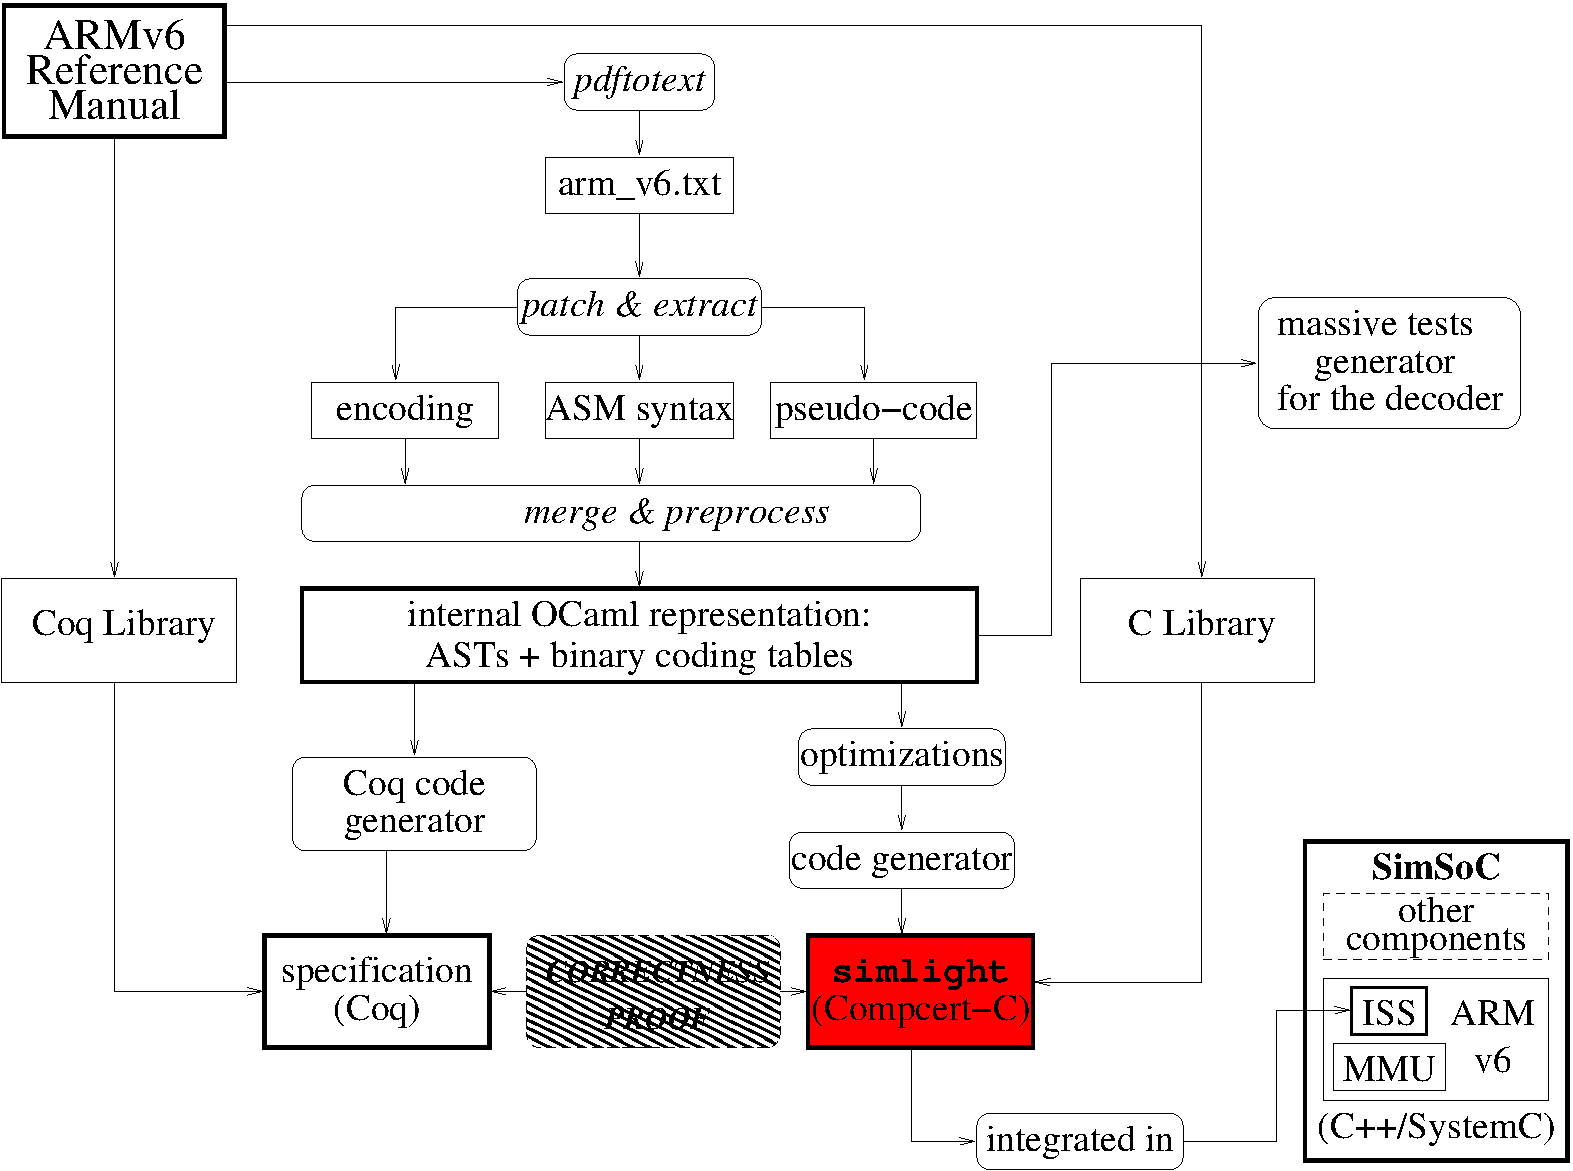
\includegraphics[width=.9\linewidth]{fig/highlight_concrete.pdf}
\end{frame}

\begin{frame}
\frametitle{Ways of generating C code}
\begin{center}
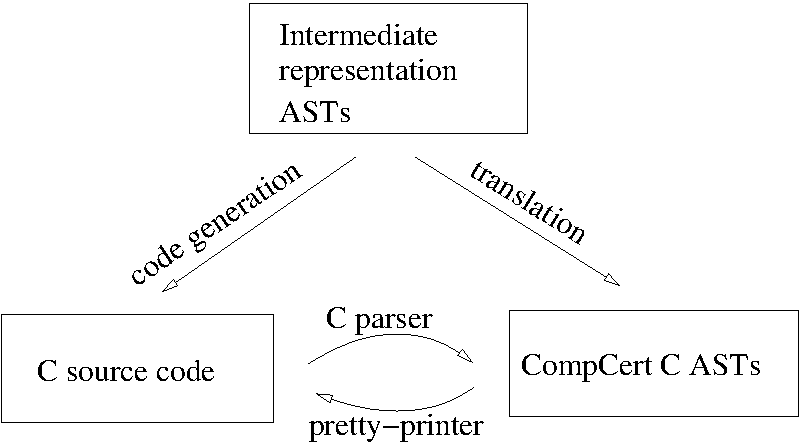
\includegraphics[width=.85\linewidth]{fig/genc.pdf}
\end{center}
\end{frame}

\begin{frame}[fragile]
\frametitle{C source code of ARM instruction ADC}
\small
\begin{alltt}
void ADC(struct SLv6_Processor *proc,\scriptsize
    const bool S,
    const SLv6_Condition cond,
    const uint8_t d,
    const uint8_t n,
    const uint32_t shifter_operand)
\{ \small
 const uint32_t old_Rn = reg(proc,n);
 \bleu{if} (ConditionPassed(&proc->cpsr, cond)) \{
   set_reg_or_pc
     (proc,d,((old_Rn+shifter_operand)+proc->cpsr.C_flag));
   \bleu{if} (((S == 1) && (d == 15))) \{ \tiny
     \bleu{if} (CurrentModeHasSPSR(proc))
       copy_StatusRegister(&proc->cpsr, spsr(proc));
     \bleu{else}
       unpredictable();
   \} \bleu{else} \{
     \bleu{if} ((S == 1)) \{
       proc->cpsr.N_flag = get_bit(reg(proc,d),31);
       proc->cpsr.Z_flag = ((reg(proc,d) == 0)? 1: 0);
       proc->cpsr.C_flag = CarryFrom_add3(old_Rn, shifter_operand, proc->cpsr.C_flag);
       proc->cpsr.V_flag = OverflowFrom_add3(old_Rn, shifter_operand, proc->cpsr.C_flag);
      \}
    \}
  \}
\}
\end{alltt}
\end{frame}

\begin{frame}[fragile]
\frametitle{Coq representation of CompcertC AST of ADC}
\newcommand{\mycirc}{\begin{math}\circ\end{math}}
\newcommand{\tbs}{\textbackslash}
\newcommand{\mabullet}{\begin{math}\bullet\end{math}}
\small
\begin{alltt}
Definition ADC\_Coq\_simlight := (ADC, Internal 
    \{| fn_return := void; fn_params := \tiny
         [proc -: `*` typ_SLv6_Processor; 
          S -: uint8; cond -: int32; d -: uint8; n -: uint8; 
          shifter_operand -: uint32];
         fn_vars := [ old_Rn -: uint32];\small
      fn_body :=
($ old_Rn`:\mycirc) `= (call (\tbs{}reg`:\mycirc) E[\tbs{}proc`:\mycirc; \tbs{}n`:\mycirc] \mycirc)`:\mycirc;;
\bleu{`if}\,(\mabullet\,(\tbs{}ConditionPassed`:\mycirc)\,E[&((`*(\tbs{}proc`:\mycirc)`:\mycirc)|cpsr`:\mycirc)`:\mycirc;\,\tbs{}cond`:\mycirc] \mycirc)
 \bleu{then} (\mabullet\,(\tbs{}set_reg_or_pc`:\mycirc) E[\tbs{}proc`:\mycirc; \tbs{}d`:\mycirc; ((\tbs{}old_Rn`:\mycirc)+\mabullet)+\mabullet:\mycirc]\,\mycirc);;
 \bleu{`if} ((($ S`:\mycirc)==(#1`:\mycirc)`:\mycirc)&(($ d`:\mycirc)==(#15`:\mycirc)`:\mycirc)`:\mycirc)\tiny
     \bleu{then} \bleu{`if} (call (\tbs{}CurrentModeHasSPSR`:\mycirc) E[\tbs{}proc`:\mycirc] \mycirc)
      \bleu{then} (call (\tbs{}copy_StatusRegister`:\mycirc) E[&(\mabullet|cpsr`:\mycirc)`:\mycirc; \mabullet] \mycirc)
      \bleu{else} (call ($ unpredictable`:\mycirc) E[] \mycirc)
     \bleu{else} \bleu{`if} (($ S`:\mycirc)==(#1`:\mycirc)`:\mycirc)
      \bleu{then} ((($ proc`:\mycirc)|cpsr`:\mycirc)|N_flag`:\mycirc) `= 
       (\mabullet\,(\tbs{}get_bit`:\mycirc) E[(\mabullet\,(\tbs{}reg`:\mycirc) E[\tbs{}proc`:\mycirc; \tbs{}d`:\mycirc] \mycirc); #31`:\mycirc] \mycirc)`:\mycirc;;
           ((($ proc`:\mycirc)|cpsr`:\mycirc)|Z_flag`:\mycirc) `= 
       (((\mabullet (\tbs{}reg`:\mycirc) \mabullet \mycirc)==(#0`:\mycirc)`:\mycirc)?(#1`:\mycirc)`:(#0`:\mycirc)`:\mycirc)`:\mycirc;;
           ((($ proc`:\mycirc)|cpsr`:\mycirc)|C_flag`:\mycirc) `= 
       (\mabullet (\tbs{}CarryFrom_add3`:\mycirc) E[\mabullet; \mabullet; (\mabullet (\mabullet|C_flag`:\mycirc) \mycirc)] \mycirc)`:\mycirc;;
           ((($ proc`:\mycirc)|cpsr`:\mycirc)|V_flag`:\mycirc) `= 
       (\mabullet (\tbs{}OverflowFrom_add3`:\mycirc) E[(\mabullet (\tbs{}old_Rn`:\mycirc) \mycirc); \mabullet; \mabullet] \mycirc)`:\mycirc
   \bleu{else} skip
 \bleu{else} skip |\}).
\end{alltt}
\end{frame}
%$

%%%%%%%%%%%%%%%%%%%%%%%%%%%%%%%%%%%%%%%%%%%
\section{Correctness proof of ARMv6 instruction}

%%%%%%%%%%%%%%%%%%%%%%%%%%%%%%%%%%%%%%%%%%%


\begin{frame}
\frametitle{Main theorem for ADC}
\hfil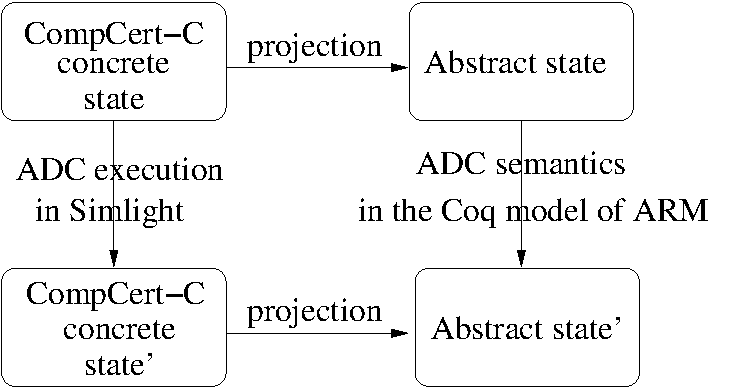
\includegraphics[width=.85\linewidth]{fig/theorem.pdf}
\end{frame}

\subsection{Differences between the two representations}
\begin{frame}
\frametitle{Differences between the two representations}
\begin{block}{Different data types}
More complex types in Simlight, for example:\\
Coq model: CPSR = 32 bits word\\
Simlight: CPSR = data structure, 1 byte-field for every significant bit
\end{block}
\begin{block}{Different semantics}
Coq specification: semantics = function\\
Compcert-C: big-step operational semantics = relation
\end{block}
\begin{block}{Different memory models}
Coq model: on a direct representation of processor state\\
Compcert-C: on a C memory state where processor state is stored
\end{block}
\end{frame}

\begin{frame}[fragile]
\frametitle{Differences between the two representations}
\begin{block}{CPSR = SPSR}
\begin{itemize}
\item Coq specification:
\begin{alltt}
set_cpsr (spsr st em)
\end{alltt}
\item C source code: 
\begin{alltt}
copy_StatusRegister(&proc->cpsr, spsr(proc))
\end{alltt}
\item CompCert C AST:
\begin{alltt}\small
(Ecall (Evalof (Evar \bleu{copy_StatusRegister} T14) T14)
  (Econs
    (Eaddrof
       (Efield (Ederef (Evalof (Evar proc T3) T3) T6) 
               \bleu{cpsr} T7) T8)
          (Econs
             (Ecall (Evalof (Evar \bleu{spsr} T15) T15)
                (Econs (Evalof (Evar proc T3) T3) 
                 Enil) T8) Enil)) T12)
\end{alltt}
\end{itemize}
\end{block}
\end{frame}

\subsection{Projection of ARMv6 processor state}
\begin{frame}
\frametitle{Projection of ARMv6 processor state ~~(excerpt)}
\hfil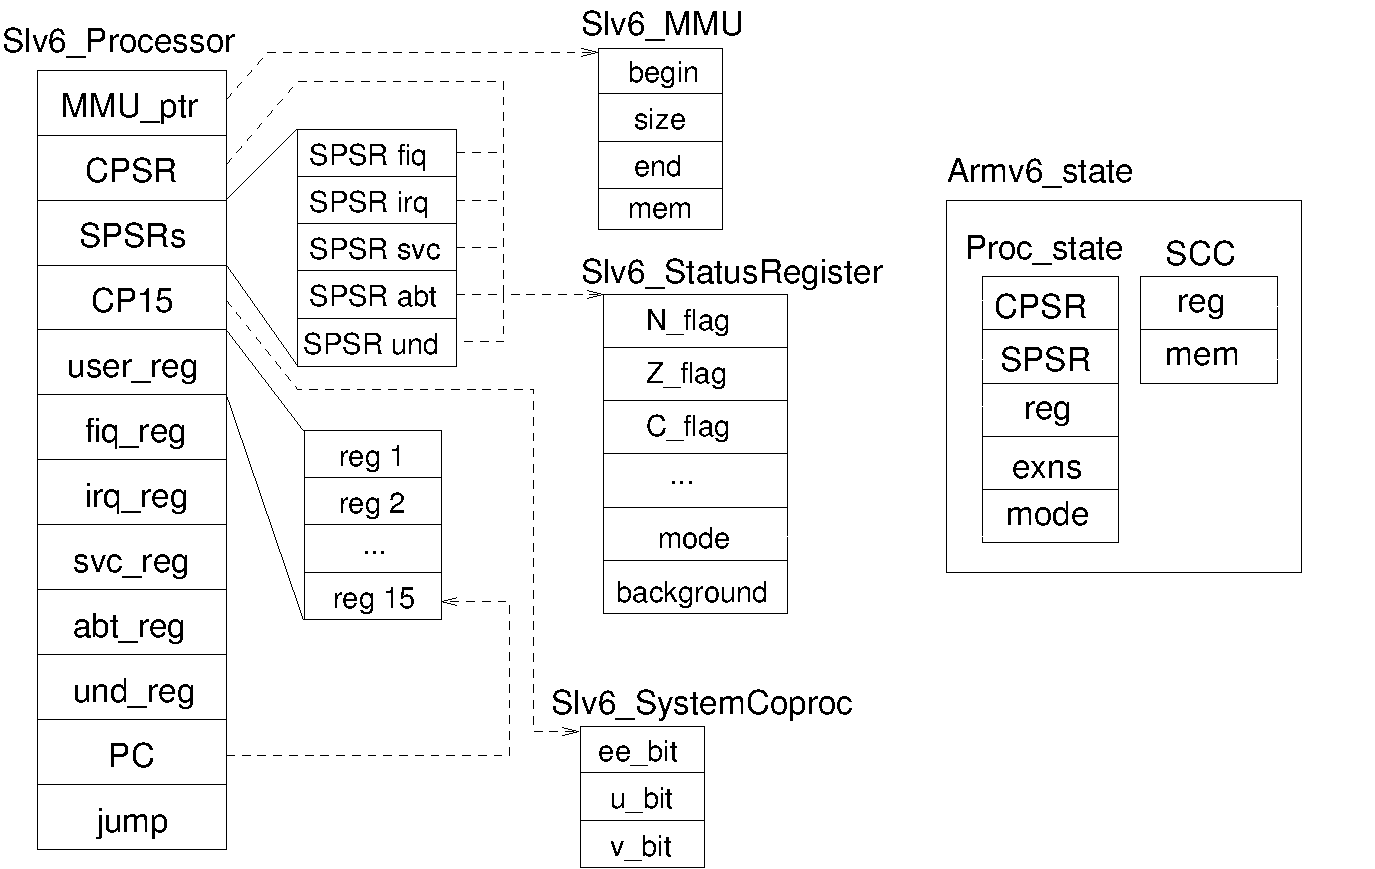
\includegraphics[width=1.01\linewidth]{fig/projection1.pdf}
\end{frame}

\begin{frame}
\frametitle{Projection of ARMv6 processor state ~~(excerpt)}
\hfil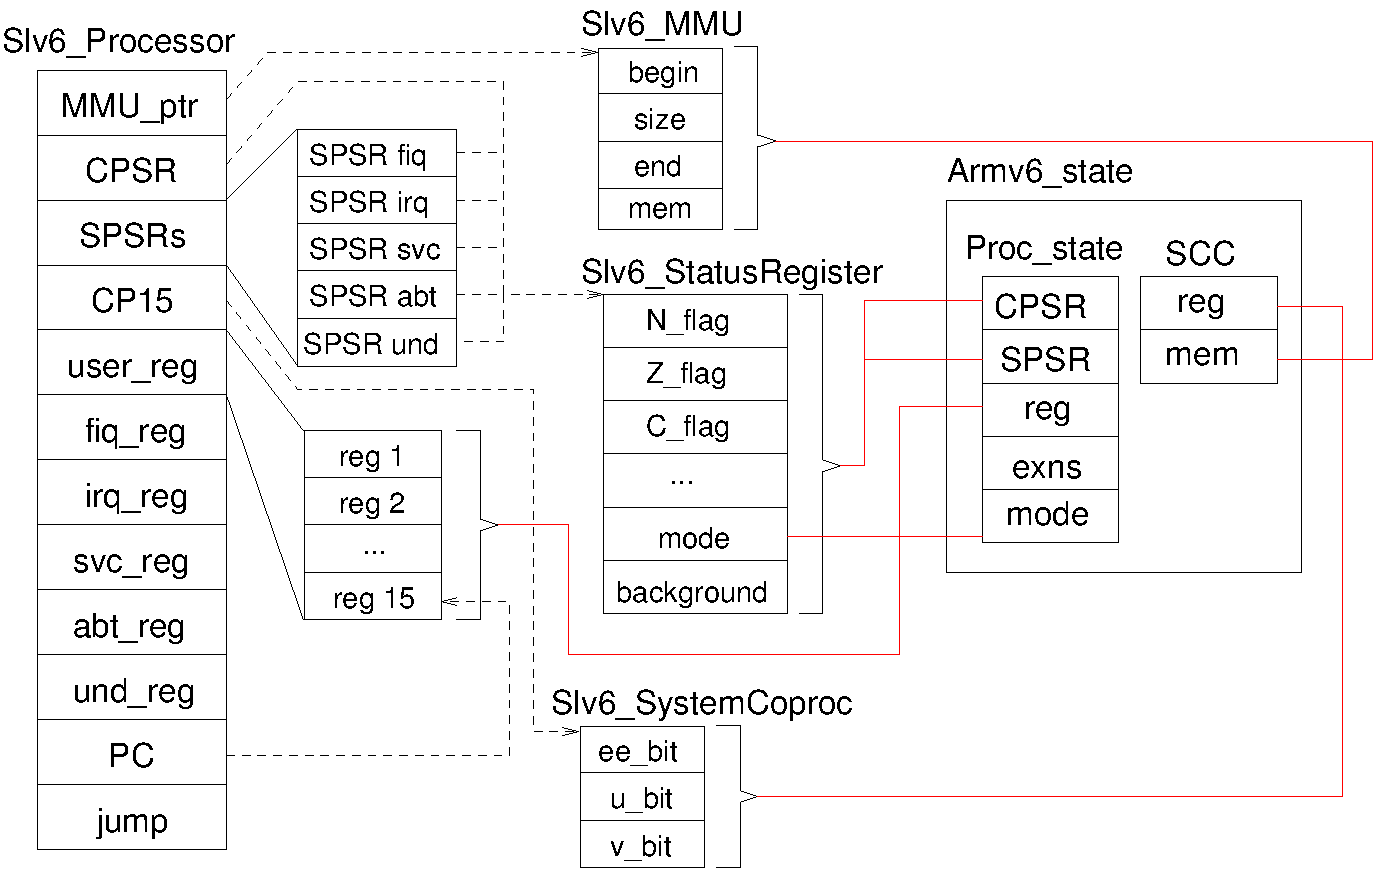
\includegraphics[width=1.01\linewidth]{fig/projection2.pdf}
\end{frame}

\begin{frame}[fragile]
\frametitle{Projection implementation}
\begin{alltt}
Definition proc_proj (m:Mem.mem) (e:env):
  Arm6_State.state:=
  Arm6_State.mk_state 
    (Arm6_Proc.mk_state 
       (\bleu{cpsr_proj} m e) 
       (\bleu{spsr_proj} m e) 
       (\bleu{regs_proj} m e) 
       nil 
       (\bleu{mode_proj} m e))
    (Arm6_SCC.mk_state 
       (\bleu{screg_proj} m e) 
       (\bleu{mem_proj} m e)).
\end{alltt}
\end{frame}

\begin{frame}[fragile]
\frametitle{Projection implementation}
\begin{block}{}
Based on the low level function \brique{\tt Mem.loadv} from CompCert C
\end{block}
\begin{alltt}
\small
Definition regs_proj (m:Mem.mem) (e:env):register->word:=
  let load_reg id n m e:=
    match find_reg m e id with 
      | Some(Vptr b ofs)=>load_val (\brique{Mem.loadv} Mint32 m 
                            (Vptr b (add ofs (repr n))))
      | _ =>Int.zero
\tiny
    end in
    fun r =>      match r with
        | R k => load_reg user_regs k m e
        | R_svc k _=> load_reg svc_regs k m e
        | R_abt k _=> load_reg abt_regs k m e
        | R_und k _=> load_reg und_regs k m e
        | R_irq k _=> load_reg irq_regs k m e
        | R_fiq k _=> load_reg fiq_regs k m e
      end.
\small
Definition \textbf{\textit{rn_related}} (m:Mem.mem)(e:env)(rn:regnum):Prop:=
  regs_proj m e n = rn.
\end{alltt}
\end{frame}

\subsection{Main theorem and lemma}
\begin{frame}[fragile]
\frametitle{Main theorem}
\begin{alltt}
\textbf{Rd = Rn + shifter_operand + C Flag;}
\end{alltt}
\begin{theorem}
\begin{itemize}
\item $G,empty\_env\vdash \texttt{alloc\_variables},\brique{M0}\overset{vars}{\Rightarrow}\brique{M1},E$
\item $G,E \vdash \texttt{bind\_parameters},\brique{M1} \overset{vargs}{\Rightarrow}\cvert{M}$
\item $\mathit{proc\_related} \: \cvert{M} \: (\texttt{Ok}\: st)$
\item similarly for the arguments of \texttt{ADC}:\\
  bit\_related \cvert{M} \:  sbit\\
  cond\_related \cvert{M} \: cond\\
  rd\_related \cvert{M} \: rd\\
  rn\_related \cvert{M} \: rn\\
  shifter\_operand\_related \cvert{M} \: shifter\_operand
\item 
  $G,E\vdash \texttt{ADC\_CompCertC\_AST},\cvert{M}\overset{t}{\Rightarrow}out,\cvert{M'}$
\end{itemize}
then $\mathit{proc\_related}\: \cvert{M'} \:(\texttt{ADC\_Coq}\: (\mathit{arguments},\:st))$.
\end{theorem}
\end{frame}

\begin{frame}
\frametitle{Lemmas on internal function (example: CarryFrom\_add3)}The concrete model simulates the abstract model.
% JF -> XM : the previous sentence may be better on the next slide?
\begin{lem}
\begin{itemize}
\item $\mathit{bit\_related} \:\cvert{M} \: \bleu{Cbit}$
\item $\mathit{rn\_related} \:\cvert{M} \: \bleu{rn}$
\item $\mathit{shifter\_operand\_related} \:\cvert{M} \: \bleu{shifter\_operand}$
\item $G,E\vdash \texttt{CarryFrom\_add3\_CompCertC\_AST},\cvert{M}\overset{t}{\Rightarrow}v,\cvert{M}'$
\end{itemize}
then $v~=~\texttt{CarryFrom\_add3\_Coq}~\bleu{rn~shifter\_operand~Cbit}$.
\end{lem}
\end{frame}

\begin{frame}
\frametitle{Lemmas on internal function (example: CarryFrom\_add3)}
The evaluation results of the abstract model and the concrete model are equivalent.
%After evaluating the function, the projection of the key variables (e.g. proc) still holds.
\begin{lem}
\begin{itemize}
\item $\mathit{proc\_related} \: \cvert{M} \: (\texttt{Ok}\: \bleu{st})$
\item $G,E\vdash \texttt{CarryFrom\_add3\_CompCertC\_AST},\cvert{M}\overset{t}{\Rightarrow}v,\cvert{M}'$
\end{itemize}
then $\mathit{proc\_related} \: \cvert{M'} \: (\texttt{Ok}\: \bleu{st})$.
\end{lem}
\end{frame}

\subsection{CompCert C semantics}
\begin{frame}
\frametitle{CompCert C semantics}
\begin{block}{eval\_assign}
\begin{equation}
\frac
{\begin{array}{c}
G,E\vdash l~M\xLongrightarrow{t1}l',M1\qquad
G,E\vdash r~M1\xLongrightarrow{t2}r',M2\\
G,E\vdash l'~M2\Rightarrow (b, ofs)\qquad
G,E\vdash r'~M2\Rightarrow v\\
cast(v,typeof(l),typeof(r))=~\lfloor v'\rfloor\\
store (G,~typeof(l),~M2,~(b,ofs),~v)=~\lfloor M3\rfloor\\
\end{array}
}
{G,E\vdash (l=r)~M\xLongrightarrow{t1**t2**t3}v',M3}
\end{equation}
\end{block}
\begin{block}{eval\_funcall}
\begin{equation}
\frac
{\begin{array}{c}
G,E\vdash rf~M~\xLongrightarrow{t1}~rf',M1\qquad
G,E\vdash rarg^*~M1~\xLongrightarrow{t2}~rarg'^*,M2\\
G,E\vdash M2~rf' \Rightarrow vf\qquad
\texttt{find\_funct}~(G,vf)~=~\lfloor fd\rfloor\\
\vdash M2~fd~varg^* \xLongrightarrow{t3}vres,M3
\end{array}
}
{G,E\vdash M~\langle\textrm{\texttt{Call}}\rangle\xLongrightarrow{t1**t2**t3}vres,M3}
\end{equation}
\end{block}
\end{frame}

\section{Handcrafted Inversions Made Operational on Operational Semantics}
\begin{frame}
\frametitle{Issue: handling large inversion}

Correctness proofs based on an operational semantics $\Rightarrow$ \\
reasoning on hypotheses relating objects 
according to this semantics

\medskip

Technically: semantics = inductive type $~\Rightarrow~$ inversion

\medskip

\begin{itemize}
\item
  CompCert C operational semantics : many large rules
\item
  For Simlight : inversions \brique{all over the place!}
\item 
  Coq \texttt{inversion} : \brique{efficiency} and \brique{controllability} issues
\end{itemize}

\medskip

Solution: build our own tactic ~ \bleu{\hcinv} ~ [ITP'13]

\end{frame}

\begin{frame}
\frametitle{What is an inversion}
\begin{block}{Inversion}
An inversion is a kind of forward reasoning step that allows for users to extract all useful information contained in a hypothesis whose type is defined using constructors -- inductive or coinductive predicates.
\end{block}
\end{frame}


\begin{frame}[fragile]
\frametitle{A toy language}
\small
\begin{alltt}
Inductive tm : Type :=
  | tm_const : nat -> tm
  | tm_plus : tm -> tm -> tm.

Inductive val : Type :=
  | nval  : nat -> val
  | bval  : bool -> val.

Inductive eval : tm -> val -> Prop :=
  | E_Const : forall n,
      eval (tm_const n) (nval n)
  | E_Plus : forall t1 t2 n1 n2,
      eval t1 (nval n1) ->
      eval t2 (nval n2) ->
      eval (tm_plus t1 t2) (nval (plus n1 n2)).
\end{alltt}
\end{frame}

\begin{frame}[fragile]
\frametitle{Using inversion}
\small
\begin{alltt}
Inductive eval : tm -> val -> Prop :=
  | E_Const : forall n,
      \bleu{eval} (\cvert{tm_const} n) (nval n)
  | E_Plus : forall t1 t2 n1 n2,
      eval t1 (nval n1) ->
      eval t2 (nval n2) ->
      \bleu{eval} (\brique{tm_plus} t1 t2) (nval (plus n1 n2)).
\end{alltt}
Consider the goal:

\begin{alltt}
e : \bleu{eval} (\brique{tm_plus} (tm_const 1) (tm_const 2)) v
============================
v = nval 3
\end{alltt}

\end{frame}


\begin{frame}[fragile]
\frametitle{Using inversion}
\small
\begin{alltt}
e : eval (tm_plus (tm_const 1) (tm_const 2)) v
============================
v = nval 3
\end{alltt}
Using Coq built-in inversion:
\begin{alltt}
\bleu{inversion e; subst.}
...
\brique{H1} : eval (tm_const 1) (nval n1)
\brique{H3} : eval (tm_const 2) (nval n2)
============================
nval (n1 + n2) = nval 3
\end{alltt}
\end{frame}

%\subsection{Issue from CompCert C semantics}
\begin{frame}[fragile]
\frametitle{Issue from CompCert C semantics}
\small
\begin{alltt}
H:eval_expr (Genv.globalenv prog_adc) e m RV
   (Ecall (Evalof (Evar copy_StatusRegister T14) T14)
      (Econs
         (Eaddrof
            (Efield (Ederef (Evalof (Evar proc T3) T3) T6)
              adc_compcert.cpsr T7) T8)
         (Econs
            (Ecall (Evalof (Evar spsr T15) T15)
               (Econs (Evalof (Evar proc T3) T3) Enil) T8)
                Enil))
      T12) t m' a'
============================
   proc_state_related m' e st'
\end{alltt}
\begin{alltt}
\brique{
  inv H. inv H4. inv H9. inv H5. inv H4. inv H5. 
  inv H15. inv H4. inv H5. inv H14. inv H4. inv H3. 
  inv H15. inv H5. inv H4. inv H5. inv H21. inv H13.
  ...}
\end{alltt}
\end{frame}
\begin{frame}


\frametitle{Well-known disadvantage of original inversion}
\begin{block}{Disadvantage}
\begin{itemize}
\item Basic inversion: no control on generated names, scripts are \brique{unmanageable} during maintenance.
\item
If we want to control variables and hypothesis names using \texttt{inversion...as...},
we have to manually give \brique{a lot of names}.
\item
The underlying proof term is complicated \\ 
$\fl$ \brique{time consuming} when designing the script.
\item
Especially harmful:
for most C expressions, inversion needed \brique{many times} 
to find the relation between memories \texttt{\Large m} and \texttt{\Large m'}.
\end{itemize}
\end{block}
\end{frame}

\subsection{General design concept}

\begin{frame}
\frametitle{Our hand crafted inversion (hc\_inversion)}
\large
\begin{itemize}
\item diagonalization function
\item dedicated Ltac definition 
\end{itemize}
\bigskip
Easy to tune
\end{frame}

\begin{frame}[fragile]
\frametitle{The diagonalization function}
\begin{itemize}
\item \cvert{yields the premises of focused constructor}
\item %\bleu{independent from specific conclusion}
\item %\brique{relates identifiers for the same variable in premise and conclusion}
\end{itemize}
For constructor E\_Plus:
\begin{alltt}
\textbf{diag} t v := match t with
  | tm_plus tc1 tc2 =>
      forall X: tm -> Prop,
        (\cvert{\(\forall\) n1 n2, eval tc1 (nval n1) ->
                  eval tc2 (nval n2)} -> 
                  X (nval (plus n1 n2))) -> X \brique{v}
  | _ => True
end
\end{alltt}
\end{frame}

\begin{frame}[fragile]
\frametitle{The diagonalization function}
\begin{itemize}
\item \cvert{yields the premises of focused constructor}
\item \bleu{independent from specific conclusion}
\item %\brique{relates identifiers for the same variable in premise and conclusion}
\end{itemize}
For constructor E\_Plus:
\begin{alltt}
\textbf{diag} t v := match t with
  | tm_plus tc1 tc2 =>
      \bleu{forall X: tm -> Prop,}
        (\cvert{\(\forall\) n1 n2, eval tc1 (nval n1) ->
                  eval tc2 (nval n2)} -> 
                  \bleu{X} (nval (plus n1 n2))) -> \bleu{X} \brique{v}
  | _ => True
end
\end{alltt}
\end{frame}

\begin{frame}[fragile]
\frametitle{The diagonalization function}
\begin{itemize}
\item \cvert{yields the premises of focused constructor}
\item \bleu{independent from specific conclusion}
\item \brique{relates identifiers for the same variable in premise and conclusion}
\end{itemize}
For constructor E\_Plus:
\begin{alltt}
\textbf{diag} t v := match t with
  | tm_plus tc1 tc2 =>
      \bleu{forall X: tm -> Prop,}
        (\cvert{\(\forall\) n1 n2, eval tc1 (nval n1) ->
                  eval tc2 (nval n2)} -> 
                  \bleu{X} \brique{(nval (plus n1 n2))}) -> \bleu{X} \brique{v}
  | _ => True
end
\end{alltt}
\end{frame}

\begin{frame}[fragile]
\frametitle{The dedicated Ltac definition}
\small
\begin{alltt}
Definition \bleu{pr_plus_1} \{t\} \{v\} (e: eval t v) :=
  match e in (eval t v) return \textbf{diag} t v with
    | E_Plus _ _ n1 n2 e1 e2 => (fun X k => k n1 n2 e1 e2)
    | _ => I
  end.
\end{alltt}
\medskip
\begin{alltt}
e : eval (tm_plus (tm_const 1) (tm_const 2)) v
============================
v = nval 3
\end{alltt}
Using hand crafted inversion
\begin{alltt}
\bleu{apply (pr_plus_1 e); intros n1 n2 e1 e2.}
...
\cvert{e1} : eval (tm_const 1) (nval n1)
\cvert{e2} : eval (tm_const 2) (nval n2)
============================
nval (n1 + n2) = nval 3
\end{alltt}
\end{frame}

\subsection{Using our hand-crafted inversion in SimSoC-Cert}

% \begin{frame}[fragile]
% \frametitle{Recall the evaluation rule of a field in CompCert C semantics}
% The evaluation rule of a field in CompCert C semantics:
% \begin{alltt}
% \small
% Inductive eval_expr :
%   env-> mem-> kind-> expr-> trace-> mem-> expr-> Prop:=
%   ...
%   | eval_field : \(\forall\) e m a t m' a' f ty,
%      eval_expr e m RV a t m' a' ->
%      eval_expr e m LV (Efield a f ty) t m' (Efield a' f ty)
% \end{alltt}
% \end{frame}

% \begin{frame}[fragile]
% \frametitle{Inversion rule for eval\_field}
% \small
% \begin{alltt}
% Definition inv_field {g} {e} {m} {ex} {t} {m'} {ex'}
%   (ee:eval_expr g e m LV ex t m' ex') :=
%   let diag e ex ex' m m' :=
%     match ex with
%       | Efield a b c =>
%         \(\forall\) (X:expr->Prop),
%         (\(\forall\) t a', eval_expr g e m RV a t m' a' -> 
%                            X (Efield a' b c)) -> X ex'
%       | _ => True
%     end in
%     match ee in (eval_expr _ e m _ ex _ m' ex')
%              return  diag e ex ex' m m'  with
%       | eval_field _ _ _ t _ a' _ _ H1 => 
%           fun X k => k t a' H1
%       | _ => I
%     end.
% \end{alltt}
% \end{frame}

% \begin{frame}[fragile]
% \frametitle{High-level tactic for inductive type \texttt{eval\_expr}}
% \small
% \begin{alltt}
% Ltac inv_eval_expr m m' :=
%   ...
%   let t1_:=fresh "t" in
%   let v1_:=fresh "v" in
%   let ev_ex1 := fresh "ev_ex" in
%   ...
%   match goal with
%   ...
%   |[ee: eval_expr ?ge ?e m LV (Efield ?a ?f ?ty) ?t m' ?a' 
%       |- ?cl] =>
%       apply (inv_field ee); 
%       clear ee; intros t1_ a1_ ev_ex1; 
%       intros;
%       inv_eval_expr m m'
% \end{alltt}
% \end{frame}


\begin{frame}[fragile]
\frametitle{High-level tactic for inductive type \texttt{eval\_expr}}
\begin{block}{\texttt{inv\_eval\_expr}}
\begin{itemize}
\item 
find automatically the hypothesis we want
to invert; %by matching the targetted memory states;
\item 
revert related hypotheses;
\item 
\brique{call the right diagonalization function;}
%(all auxiliary functions are gathered in the tactic);
\item 
give meaningful names to derived variables and hypotheses;
\item 
update all other related hypotheses;% according to the new names
%and new values;
\item 
clean up useless variables and hypotheses;
\item 
repeat the steps above.% until all transitions between
%the two targetted memory states are discovered. 
\end{itemize}
\end{block}
\end{frame}

\begin{frame}[fragile]
\frametitle{hc\_inversion on the previous example}
\small
\begin{alltt}
H:eval_expr (Genv.globalenv prog_adc) e \bleu{m} RV
   (Ecall (Evalof (Evar copy_StatusRegister T14) T14)
      (Econs
         (Eaddrof
            (Efield (Ederef (Evalof (Evar proc T3) T3) T6)
              adc_compcert.cpsr T7) T8)
         (Econs
            (Ecall (Evalof (Evar spsr T15) T15)
               (Econs (Evalof (Evar proc T3) T3) Enil) T8)
                Enil))
      T12) t \bleu{m'} a'
============================
   proc_state_related m' e st'
\end{alltt}
\begin{alltt}
\brique{
  inv H. inv H4. inv H9. inv H5. inv H4. inv H5. 
  inv H15. inv H4. inv H5. inv H14. inv H4. inv H3. 
  inv H15. inv H5. inv H4. inv H5. inv H21. inv H13.
  ...}
\end{alltt}
\end{frame}

\begin{frame}[fragile]
\frametitle{hc\_inversion on the previous example}
\small
\begin{alltt}
H:eval_expr (Genv.globalenv prog_adc) e \bleu{m} RV
   (Ecall (Evalof (Evar copy_StatusRegister T14) T14)
      (Econs
         (Eaddrof
            (Efield (Ederef (Evalof (Evar proc T3) T3) T6)
              adc_compcert.cpsr T7) T8)
         (Econs
            (Ecall (Evalof (Evar spsr T15) T15)
               (Econs (Evalof (Evar proc T3) T3) Enil) T8)
                Enil))
      T12) t \bleu{m'} a'
============================
   proc_state_related m' e st'
\end{alltt}
\begin{alltt}
  \cvert{inv_eval_expr} \bleu{m m'}.
\end{alltt}
\end{frame}

\subsection{validation}
\begin{frame}\frametitle{Comparing our hand-crafted inversion with Coq built-in inversions}
\begin{table}[t]
\small
\centering
\caption{Time costs (in seconds)}
\label{t:timing}
\begin{tabular}{|l|c|c|c|c|}
\hline
 & \texttt{inversion} & \texttt{D. Inversion} & \texttt{BasicElim} & \texttt{hc\_inversion} \\
\hline
%Full example & 1.628102 & 0.976061 & 1.428089 & 0.31202 \\
Full ex. & 1.628 & 0.976 & 1.428 & \cvert{0.312} \\
\hline
%Ecall & 0.132009 & 0.076004 & 0.112007 &  0.028002\\
Ecall & 0.132 & 0.076 & 0.112 &  \cvert{0.028}\\
\hline
%Evalof &  0.132008 & 0.072004 & 0.092005 & 0.020001\\
Evalof &  0.132 & 0.072 & 0.092 & \cvert{0.020}\\
\hline
%Evar &  0.128008 & 0.064004 & 0.084006 & 0.024001\\
Evar &  0.128 & 0.064 & 0.084 & \cvert{0.024}\\
\hline
%Eaddrof &  0.140009 & 0.076005 & 0.104007 & 0.020001\\
Eaddrof &  0.140 & 0.076 & 0.104 & \cvert{0.020}\\
\hline
\end{tabular}
\end{table}

\begin{table}[t]
\small
\centering
\caption{Size of compilation results (in KBytes)}
\label{t:size}
\begin{tabular}{|l|c|c|c|c|}
\hline
 & \texttt{inversion} & \texttt{D. Inversion} & \texttt{BasicElim} & \texttt{hc\_inversion} \\
\hline
%Full example & 191346 & 459613 & 170821 & 36712\\
Full ex. & 191 & 460 & 171 & \cvert{37}\\
\hline
\end{tabular}
\end{table}
\small
   D. Inversion = Derived Inversion
\end{frame}

%%%%%%%%%%%%%%%%%%%%%%%%%%%%%%%%%%%%%%%%%%
\section{Conclusion}

%%%%%%%%%%%%%%%%%%%%%%%%%%%%%%%%%%%%%%%%%%%

\begin{frame}
\frametitle{Future work}
\begin{itemize}
\item Extend the work to the full set of instructions (136 instructions left)
\item Proofs for decoder
\item Proofs for simulation loop
\item Consider the optimized version Simlight2
\item Reuse approach in another project CCCBIP
\end{itemize}
\end{frame}

\begin{frame}
\frametitle{Size of development}
\small
\begin{table}[t]
  \centering
  \begin{tabular}{|l|r@{~}|}
    \hline
    Original ARM ref man (txt)           & 49655 \\
    ARM Parsing to an OCaml AST         & \bleu{1068} \\
    Generator (Simgen) for ARM         &   \bleu{10675} \\ 
    General C libraries on ARM         & \bleu{1852} \\ 
    General Coq libraries on ARM         & \bleu{1569} \\ 
    Generated C code for Simlight ARM operations   & \cvert{6681} \\
    Generated Coq code for ARM operations   & \cvert{2068} \\
    Generated Coq code for ARM decoding  & \cvert{592} \\
    Projection   & \bleu{857} \\
    Definition of \hcinv       & \bleu{551} \\
    Definition of other self-defined tactics      & \bleu{185}\\ 
    Proof script on ADC (2011)    & \brique{3171} \\
    Proof scripts on ADC (2012)    & \brique{1204} \\     
%% Xiaomu: please complete
    Proof script on auxiliary functions   & \brique{856} \\
    Proof script on BL (2012)   & \brique{437} \\
    Proof script on MRS (2012)   & \brique{322} \\
    ... & ...\\
    \hline 
  \end{tabular}
  \smallskip
  \caption{Sizes (in loc)}
\end{table}
\end{frame}


\begin{frame}
\begin{center}
{\huge THANKS}
\end{center}

\end{frame}


\end{document}
